\documentclass[11pt]{article}
\usepackage{worksheet_style}

% ---- Toggle: uncomment for filled version ----
%\worksheetfilledtrue
\begin{document}
\worksheetheader{1}{Calculus Review \& 3D Coordinate Systems}

\begin{background}
Welcome to Calculus III. Everything you learned in Calc I and II---limits, derivatives, integrals, Taylor series---was about functions of a single variable. This semester, we generalize all of it to functions of two, three, or more variables. Today we start with a rapid review of the tools you'll need, then introduce the 3D coordinate systems that let us describe points in space. By the end of the semester, you'll be integrating over surfaces and applying theorems that unify all of calculus.
\end{background}

%=============================================================
\wsection{Core Concepts}

\begin{itemize}[leftmargin=*, nosep]
  \item Limit: $\ds\lim_{x\to a}f(x) = L$ means \wbi{as $x$ approaches $a$, $f(x)$ gets arbitrarily close to $L$}{8cm}
  \item Derivative: $f'(a) = \ds\lim_{h\to 0}\frac{f(a+h)-f(a)}{h}$
  \item L'H\^opital's Rule: For $\frac{0}{0}$ or $\frac{\infty}{\infty}$: \; $\ds\lim_{x\to a}\frac{f(x)}{g(x)} = \wbs{\ds\lim_{x\to a}\frac{f'(x)}{g'(x)}}{4cm}$
\end{itemize}

%=============================================================
\wsection{Essential Rules}

\begin{formulabox}{Derivatives and Integrals}
\begin{multicols}{2}
\textbf{Derivatives:}
\begin{align*}
  (uv)' &= \wbs{u'v + uv'}{3cm} \\
  \left(\frac{u}{v}\right)' &= \wbs{\frac{u'v-uv'}{v^2}}{3cm} \\
  \frac{d}{dx}[f(g(x))] &= \wbs{f'(g(x))g'(x)}{3cm} \\
  \frac{d}{dx}[x^n] &= \wbs{nx^{n-1}}{2cm} \\
  \frac{d}{dx}[\ln(x)] &= \wbs{1/x}{2cm} \\
  \frac{d}{dx}[e^x] &= \wbs{e^x}{2cm}
\end{align*}

\columnbreak
\textbf{Integrals:}
\begin{align*}
  \int_a^b f(x)\,dx &= \wbs{F(b)-F(a)}{3cm} \\
  \int u\,dv &= \wbs{uv - \int v\,du}{3cm} \\
  \int x^n\,dx &= \wbs{\frac{x^{n+1}}{n+1}+C}{3cm} \\
  \int \frac{1}{x}\,dx &= \wbs{\ln|x|+C}{3cm} \\
  \int e^x\,dx &= \wbs{e^x+C}{3cm} \\
  \int \sin(x)\,dx &= \wbs{-\cos(x)+C}{3cm}
\end{align*}
\end{multicols}
\end{formulabox}

%=============================================================
\wsection{Taylor Series}

-- General form around $x = a$:
\[f(x) = \wbml{f(a) + f'(a)(x-a) + \frac{f''(a)}{2!}(x-a)^2 + \frac{f'''(a)}{3!}(x-a)^3 + \cdots}\]

-- Common series:
\begin{align*}
  e^x &= \wbs{1 + x + \frac{x^2}{2!} + \frac{x^3}{3!} + \cdots}{8cm} \\
  \sin(x) &= \wbs{x - \frac{x^3}{3!} + \frac{x^5}{5!} - \cdots}{8cm}
\end{align*}

%=============================================================
\wsection{3D Coordinate Systems}

\wsubsection{Rectangular Coordinates}

-- Point in 3D: $(x,y,z)$ means \wbi{$x$ units right, $y$ units forward, $z$ units up}{7cm}

\begin{formulabox}{Distance and Midpoint in 3D}
\textbf{Distance} between $(x_1,y_1,z_1)$ and $(x_2,y_2,z_2)$:
\[d = \wbml{\sqrt{(x_2-x_1)^2+(y_2-y_1)^2+(z_2-z_1)^2}}\]
\textbf{Midpoint:}
\[M = \wbml{\left(\frac{x_1+x_2}{2},\; \frac{y_1+y_2}{2},\; \frac{z_1+z_2}{2}\right)}\]
\end{formulabox}

\begin{center}
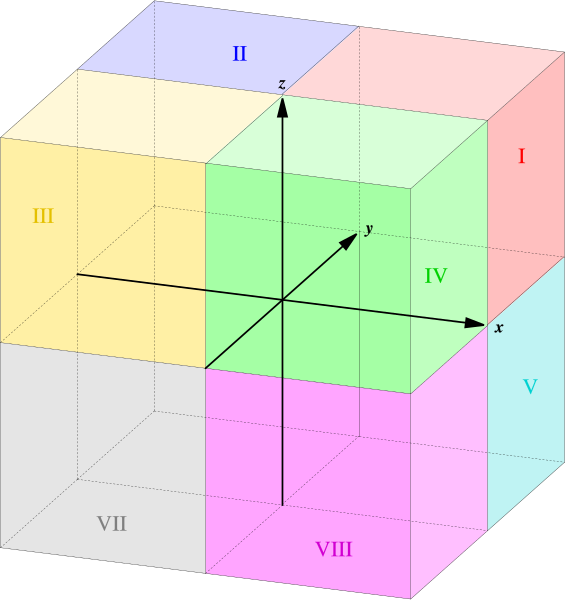
\includegraphics[width=7cm]{pics/octant.png}\\
{\small The eight octants of 3D space.}
\end{center}

-- Coordinate planes: $xy$-plane: $\wbm{z=0}$ \qquad $xz$-plane: $\wbm{y=0}$ \qquad $yz$-plane: $\wbm{x=0}$

\wsubsection{Alternative Coordinate Systems}

\begin{formulabox}{Polar and Cylindrical}
\begin{multicols}{2}
\textbf{Polar} $(r,\theta)$:
\begin{itemize}[nosep]
  \item $r$: \wbi{distance from origin}{3cm}
  \item $\theta$: \wbi{angle from $x$-axis}{3cm}
  \item To rectangular:\\
    $x = \wbm{r\cos\theta}$, \; $y = \wbm{r\sin\theta}$
  \item From rectangular:\\
    $r = \wbm{\sqrt{x^2+y^2}}$, \; $\theta = \wbm{\tan^{-1}(y/x)}$
\end{itemize}

\columnbreak
\textbf{Cylindrical} $(r,\theta,z)$:
\begin{itemize}[nosep]
  \item $r$: \wbi{distance from $z$-axis}{3cm}
  \item $\theta$: \wbi{angle from $x$-axis}{3cm}
  \item $z$: \wbi{height}{2cm}
  \item To rectangular:\\
    $x = \wbm{r\cos\theta}$, \; $y = \wbm{r\sin\theta}$, \; $z = \wbm{z}$
\end{itemize}
\end{multicols}
\end{formulabox}

\begin{center}
\tdplotsetmaincoords{65}{140}
\begin{tikzpicture}[scale=3.2, tdplot_main_coords]
\pgfmathsetmacro{\r}{0.8}
\pgfmathsetmacro{\z}{0.7}
\draw[->, thick] (0,0,0) -- (1.2,0,0) node[anchor=west] {$x$-axis};
\draw[->, thick] (0,0,0) -- (0,1.2,0) node[anchor=west] {$y$-axis};
\draw[->, thick] (0,0,0) -- (0,0,1.2) node[anchor=south] {$z$-axis};
\draw[->, blue!70!black, ultra thick] (0,0,0) -- ({\r*cos(30)},{\r*sin(30)},\z) node[anchor=south] {$(r, \theta, z)$};
\draw[dashed, blue!50] ({\r*cos(30)},{\r*sin(30)},\z) -- ({\r*cos(30)},{\r*sin(30)},0);
\draw[dashed, blue!50] ({\r*cos(30)},{\r*sin(30)},0) -- (0, 0, 0);
\draw[thick, dashed, gray] (0,0,0) circle (\r);
\draw[thick, ->, red!70] (0.6,0) arc[start angle=0, end angle=30, radius=0.6];
\node[anchor=west] at (0.35,0.05) {$\theta$};
\filldraw[blue!50] ({\r*cos(30)},{\r*sin(30)},0) circle (0.5pt) node[anchor=north east] {$(r, \theta, 0)$};
\filldraw[blue!50] ({\r*cos(30)},{\r*sin(30)},\z) circle (0.5pt);
\draw[thick, dashed, green!70!black] (0,0,0) -- ({\r*cos(30)},{\r*sin(30)},0);
\node[anchor=north east] at ({\r*cos(15)/2},{\r*sin(15)/2},0) {$r$};
\end{tikzpicture}\\
{\small A point in cylindrical coordinates $(r,\theta,z)$: radius $r$ from the $z$-axis, angle $\theta$ in the $xy$-plane, and vertical height $z$.}
\end{center}

\wsubsection{Spherical Coordinates $(\rho,\theta,\phi)$}

\begin{itemize}[leftmargin=*, nosep]
  \item $\rho$: \wbi{distance from origin}{3cm}
  \item $\theta$: \wbi{angle from $x$-axis in $xy$-plane}{4cm}
  \item $\phi$: \wbi{angle from positive $z$-axis}{4cm}
\end{itemize}

-- To rectangular:
\[x = \wbm{\rho\sin\phi\cos\theta}, \quad y = \wbm{\rho\sin\phi\sin\theta}, \quad z = \wbm{\rho\cos\phi}\]

-- From rectangular:
\[\rho = \wbm{\sqrt{x^2+y^2+z^2}}, \quad \theta = \wbm{\tan^{-1}(y/x)}, \quad \phi = \wbm{\cos^{-1}(z/\rho)}\]

\begin{center}
\tdplotsetmaincoords{60}{110}
\pgfmathsetmacro{\rvec}{.8}
\pgfmathsetmacro{\thetavec}{30}
\pgfmathsetmacro{\phivec}{60}
\begin{tikzpicture}[scale=3.5,tdplot_main_coords]
  \coordinate (O) at (0,0,0);
  \draw[thick,->] (0,0,0) -- (1,0,0) node[anchor=north east]{$x$};
  \draw[thick,->] (0,0,0) -- (0,1,0) node[anchor=north west]{$y$};
  \draw[thick,->] (0,0,0) -- (0,0,1) node[anchor=south]{$z$};
  \tdplotsetcoord{P}{\rvec}{\thetavec}{\phivec}
  \draw[-stealth,color=red] (O) -- (P) node[above right] {$\rho$};
  \draw[dashed, color=red] (O) -- (Pxy);
  \draw[dashed, color=red] (P) -- (Pxy);
  \tdplotdrawarc{(O)}{0.2}{0}{\phivec}{anchor=north}{$\theta$}
  \tdplotsetthetaplanecoords{\phivec}
  \tdplotdrawarc[tdplot_rotated_coords]{(0,0,0)}{0.5}{0}%
      {\thetavec}{anchor=south west}{$\phi$}
\end{tikzpicture}\\
{\small A point in spherical coordinates $(\rho,\theta,\phi)$: distance $\rho$ from the origin, azimuthal angle $\theta$ in the $xy$-plane, and polar angle $\phi$ measured from the $+z$-axis.}
\end{center}

%=============================================================

\begin{practice}

\prob Evaluate $\ds\lim_{x\to 0}\frac{e^x-1-x-\frac{x^2}{2}}{x^3}$.

\wans{\wbm{$\frac{1}{6}$}}

\vspace{2.5cm}

\prob Find first three terms of Taylor series for $\ln(1+x)$ at $a=0$.

\wans{\wbml{$x - \frac{x^2}{2} + \frac{x^3}{3}$}}

\vspace{2.5cm}

\prob Convert cylindrical point $(3, \pi/4, 2)$ to rectangular coordinates.

\wans{\wbml{$(3\sqrt{2}/2,\; 3\sqrt{2}/2,\; 2)$}}

\vspace{2.5cm}

\prob Find distance between points $(1,1,1)$ and $(4,5,2)$.

\wans{\wbm{$\sqrt{26}$}}

\vspace{2.5cm}

\prob Convert rectangular point $(0,2,2)$ to spherical coordinates.

\wans{\wbml{$(\rho = 2\sqrt{2},\; \theta = \pi/2,\; \phi = \pi/4)$}}

\end{practice}

\end{document}
